%=========================================================================
% fig-tuning-vectorization-convolution.tex
%=========================================================================

\begin{figure}[t]

  \centering
  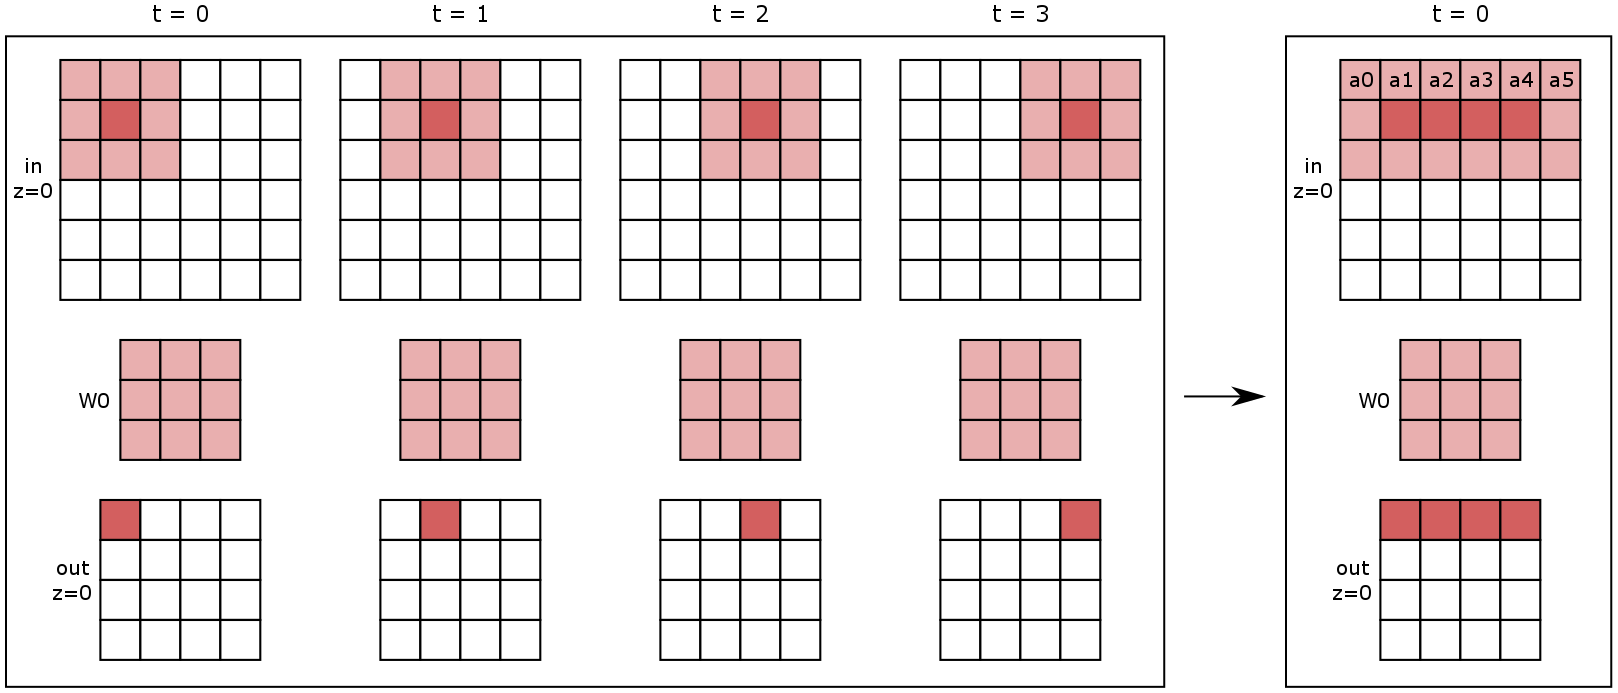
\includegraphics[width=0.9\tw]{fig-tune-vector-convolution.svg.pdf}

  \caption{\textbf{Vectorization Strategy for Convolutional Layer --} A
    6x6x1 input is convolved with a 3x3x1 filter to produce a 4x4x1 slice
    of the output. For simplicity, only one filter and the computation
    required for a single slice is shown. The box on the left illustrates
    the scalarized approach that takes four computational timesteps to
    calculate the first row of the output. The box on the
    right illustrates the vectorized approach that takes a single
    computational timestep to perform the same computations.}

  \label{fig-tuning-vectorization-convolution}

\end{figure}
